\chapter{Thiết kế hệ thống}
\section{Yêu cầu chức năng và phi chức năng}
Hệ thống cần nhận dữ liệu gốc có thể kiểm tra được, huấn luyện ba ứng viên theo cùng phép chia, chọn mô hình bằng validation, trả về xác suất hỏng qua HTTP và tạo báo cáo khi phân phối đầu vào thay đổi. Các đầu ra cần truy vết đến cấu hình, mã nguồn và tệp dữ liệu. Nhóm cũng đặt yêu cầu một người khác có thể cài phụ thuộc và chạy lại trên máy cá nhân; thiếu mô hình hoặc schema đầu vào sai phải tạo lỗi rõ ràng thay vì trả về dự đoán giả.

Về mặt phi chức năng, đây là bản mẫu học phần nên không đặt mục tiêu số yêu cầu mỗi giây hay độ trễ dịch vụ sản xuất. Tính tái tạo được kiểm tra qua seed, khóa phụ thuộc ở mức phù hợp, dấu băm dữ liệu và lệnh chạy pipeline. Tính quan sát được thể hiện qua MLflow, tệp metric và báo cáo giám sát. Tính di động được hỗ trợ bởi Python package và Docker image CPU. Tính an toàn dữ liệu ở đây tập trung vào xác thực trường đầu vào và tránh rò rỉ nhãn; hệ thống chưa có xác thực người dùng hoặc chính sách lưu trữ dữ liệu công nghiệp.

\section{Sơ đồ tổng thể}
Hình~\ref{fig:arch} mô tả đường dữ liệu và đường phục vụ. Bước \src{download} tạo CSV thô; bước \src{train} tạo mô hình, số liệu và tập tham chiếu. MLflow ghi từng lần huấn luyện vào SQLite cục bộ. API nạp cùng mô hình đã được chọn, còn công cụ monitor dùng \src{reference.csv} và một lô mới để xuất JSON trạng thái. CI chạy kiểm thử mã, độc lập với việc huấn luyện lại toàn bộ bộ dữ liệu.

\begin{figure}[H]\centering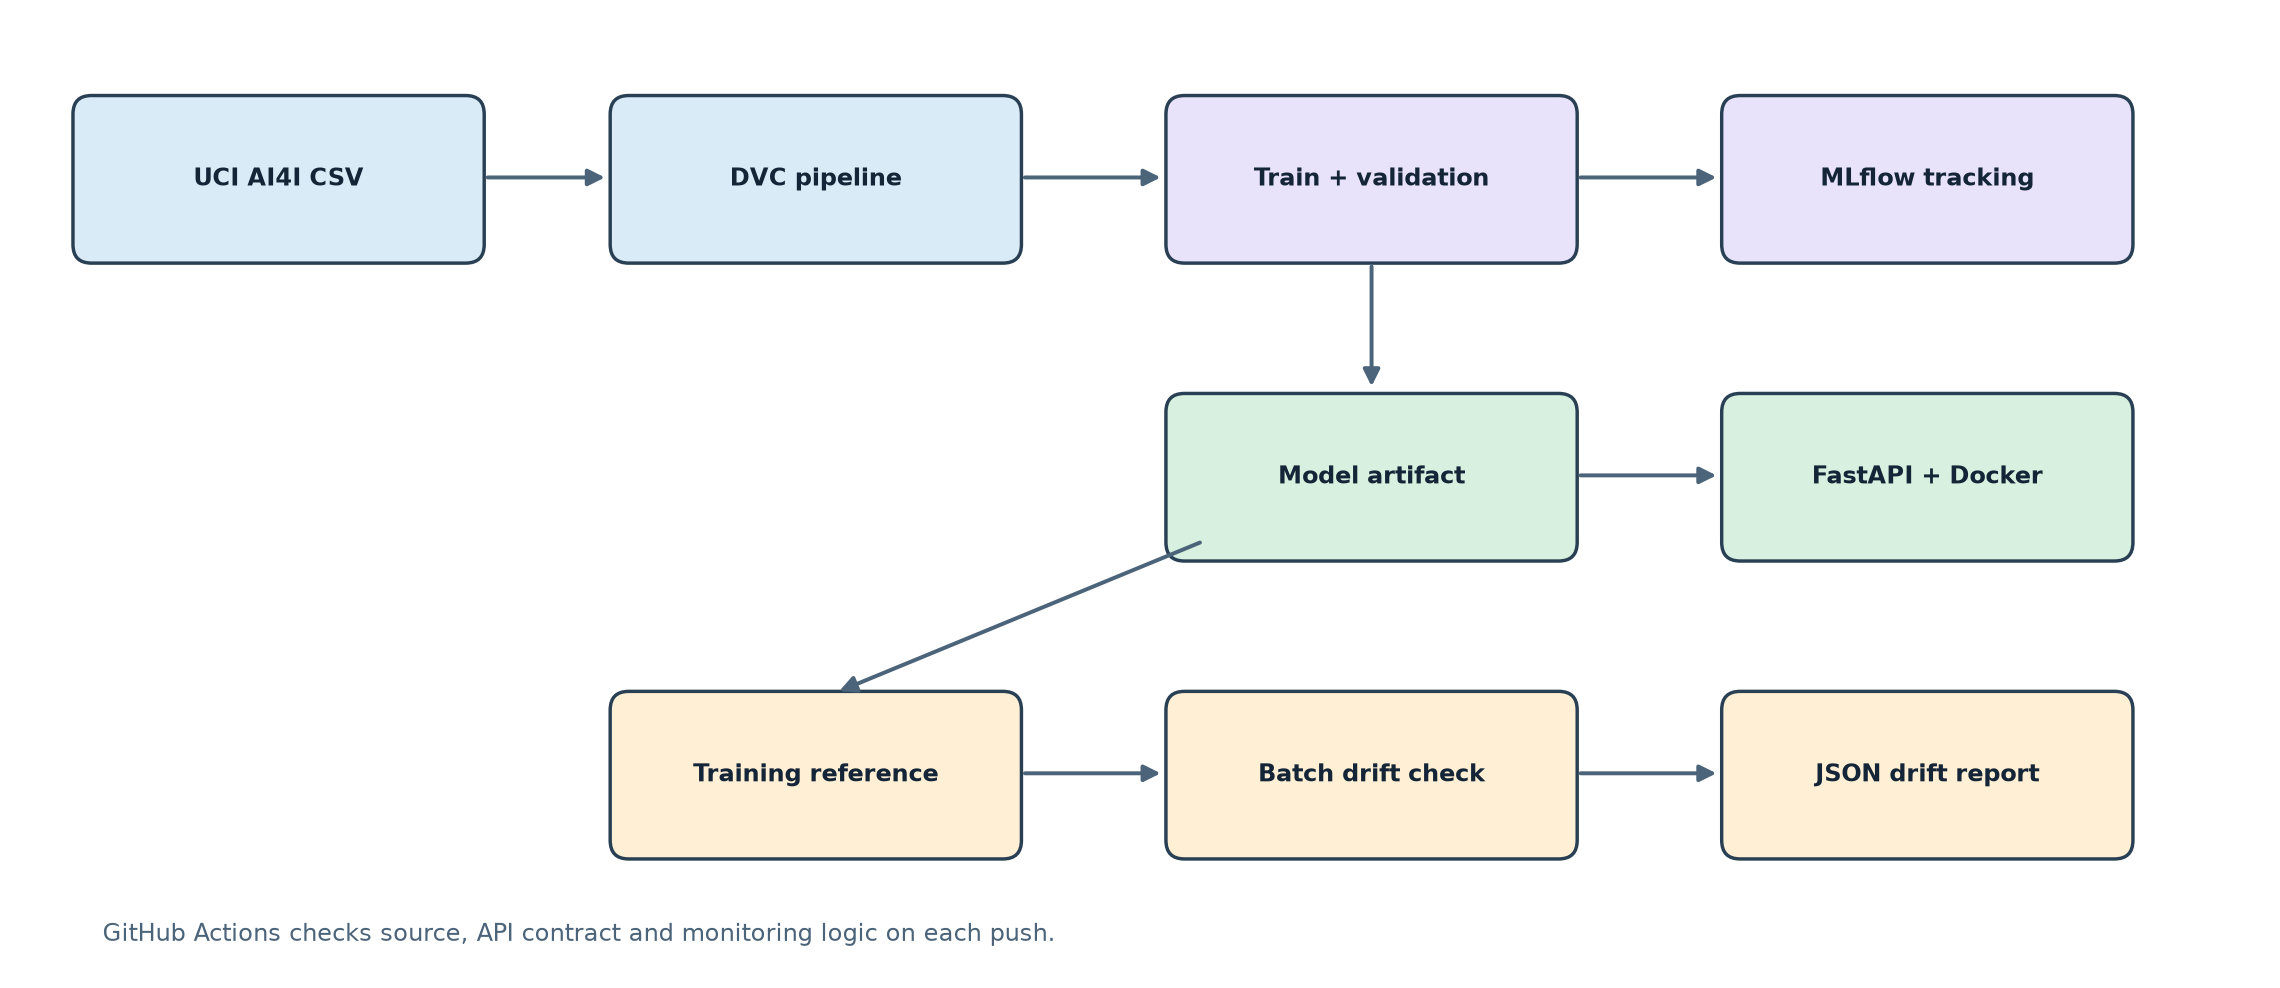
\includegraphics[width=.98\textwidth]{architecture.png}\caption{Kiến trúc triển khai của dự án. Mũi tên chỉ luồng dữ liệu hoặc hiện vật.}\label{fig:arch}\end{figure}

\section{Ranh giới các thành phần}
\src{src/predictive_maintenance/data.py} chịu trách nhiệm tải dữ liệu. \src{features.py} là hợp đồng schema huấn luyện. \src{splits.py} quy định một phép chia tập dùng chung. \src{train.py} định nghĩa tiền xử lý, ứng viên, đánh giá và xuất hiện vật. \src{api.py} nạp mô hình và nhận một bản ghi JSON; \src{monitor.py} nhận lô CSV và so sánh phân phối; \src{simulate.py} tạo dữ liệu để thử cảnh báo; \src{report.py} tổng hợp bằng chứng từ hiện vật. Phân công theo chức năng này giúp thay đổi một phần mà vẫn có thể xác định tác động đến phần khác.

Đầu ra của bước train gồm \src{model.joblib}, \src{metrics.json}, \src{reference.csv}. \src{model.joblib} chứa cả pipeline tiền xử lý, bộ phân loại, ngưỡng xác suất và danh sách sáu thuộc tính. API dùng đúng bundle này, tránh tái tạo bằng tay tiền xử lý khi triển khai. \src{metrics.json} giữ kết quả của từng ứng viên trên validation và một kết quả test của mô hình được chọn. \src{reference.csv} chỉ chứa thuộc tính của tập train, không chứa nhãn hoặc test; đây là đường chuẩn cho giám sát.

\section{Luồng huấn luyện và luồng suy luận}
Luồng huấn luyện bắt đầu từ CSV đã xác thực, chọn sáu thuộc tính, chia tập, khớp ba pipeline, ghi MLflow, chọn AP cao nhất, đánh giá test và lưu bundle. Mỗi ứng viên có cùng cách mã hóa \src{Type} và chuẩn hóa năm biến số. Đặt tiền xử lý trong pipeline làm giảm nguy cơ sử dụng thống kê từ validation hoặc test. Nếu thay đổi danh sách thuộc tính, hiện vật mô hình và hợp đồng API phải được cập nhật cùng nhau.

Luồng suy luận nhận JSON có sáu trường. Pydantic kiểm tra kiểu và miền giá trị cơ bản: \src{type} thuộc L/M/H, các nhiệt độ và tốc độ dương, mô-men xoắn và hao mòn không âm. API ánh xạ tên thân thiện của JSON sang tên cột CSV, gọi \src{predict_proba}, so sánh với ngưỡng được lưu trong bundle rồi trả về xác suất, cờ cảnh báo và ngưỡng. Điểm \src{/health} thử nạp mô hình; nếu tệp thiếu, nó trả 503. Kiểm tra này cho biết dịch vụ có nạp được hiện vật, chưa đo tính đúng đắn hay độ tươi của dữ liệu.

\section{Luồng giám sát và phản hồi}
Công cụ giám sát đọc một lô CSV, kiểm tra đủ sáu cột và số dòng tối thiểu. Với \src{Type}, nó so sánh tần suất ba giá trị; với từng biến số, nó loại giá trị không phải số hữu hạn trước phép thử KS và ghi lại số hàng lỗi. Kết quả trả về \src{ok} nếu không có thuộc tính lệch và không có lỗi chất lượng; còn lại trả \src{alert}. Cấu trúc JSON chứa chi tiết từng thuộc tính, giúp người vận hành biết cảnh báo do biến nào và do độ lệch hay do dữ liệu không hợp lệ.

Giám sát đầu vào chỉ là bước đầu của vòng phản hồi. Nếu có nhãn hỏng thật được xác nhận muộn hơn, người vận hành có thể nối dự đoán với nhãn để tính precision, recall, tỷ lệ cảnh báo và hiệu chuẩn theo thời gian. Bản mẫu chưa thực hiện bước này vì các lô demo không mô phỏng quy trình gán nhãn trễ. Một cảnh báo drift cũng không nên tự động kích hoạt huấn luyện lại: trước tiên cần kiểm tra lỗi thu thập, thay đổi thiết bị, tính hợp lệ của nhãn và kết quả trên một tập đánh giá mới.

\section{Quyết định triển khai và đánh đổi}
DVC được chọn để trình bày phụ thuộc giữa hai giai đoạn, nhưng cache chỉ có trên máy chạy, chưa cấu hình remote. MLflow dùng SQLite cục bộ, thuận tiện cho bài tập một máy nhưng không phải hạ tầng cộng tác nhiều người. Docker image chỉ cài phần phụ thuộc cần để phục vụ API, trong khi khâu huấn luyện chạy ngoài image. Cấu hình này giảm kích thước và thời gian dựng image, đồng thời đòi hỏi mô hình phải được tạo trước và gắn vào container ở chế độ chỉ đọc. Những đánh đổi này là quyết định có chủ đích theo phạm vi học phần.

